%-------------------------------------------------------------------------------
\subsubsection{Modèle cubique}
%-------------------------------------------------------------------------------

% [Exercice 2, TD2, L2 Bio SU]

\exemple{
  On considère le système
  $$
  \dot y = - y^3 + 7 y^2 - 14 y + 8.
  $$
  Ses points stationnaires sont les racines du polynôme $P(y) = - y^3 + 7 y^2 - 14 y + 8$, donc $y_1 = 1$ fait partie, donc
  $$
  P(y) = (y-1) (-y^2 + 6y + 8),
  $$
  et les deux racines de $-y^2 + 6y + 8$ sont $2$ et $4$. Les points stationnaires du système sont donc 
  $$
  y_1 = 1, \qquad y_2 = 2, \qquad y_3 = 4.
  $$
  Leur stabilité est donné par la dérivée de $P$:
  $$
  P'(y) = -3y^2 + 14 y - 14,
  $$
  soit
  $$
  P'(y_1) = -3, \qquad P'(y_2) = 2, \qquad P'(y_3) = -6.
  $$
  $y_1$ et $y_3$ sont donc des équilibres stables, et $y_2$ un équilibre instable.
  $$
  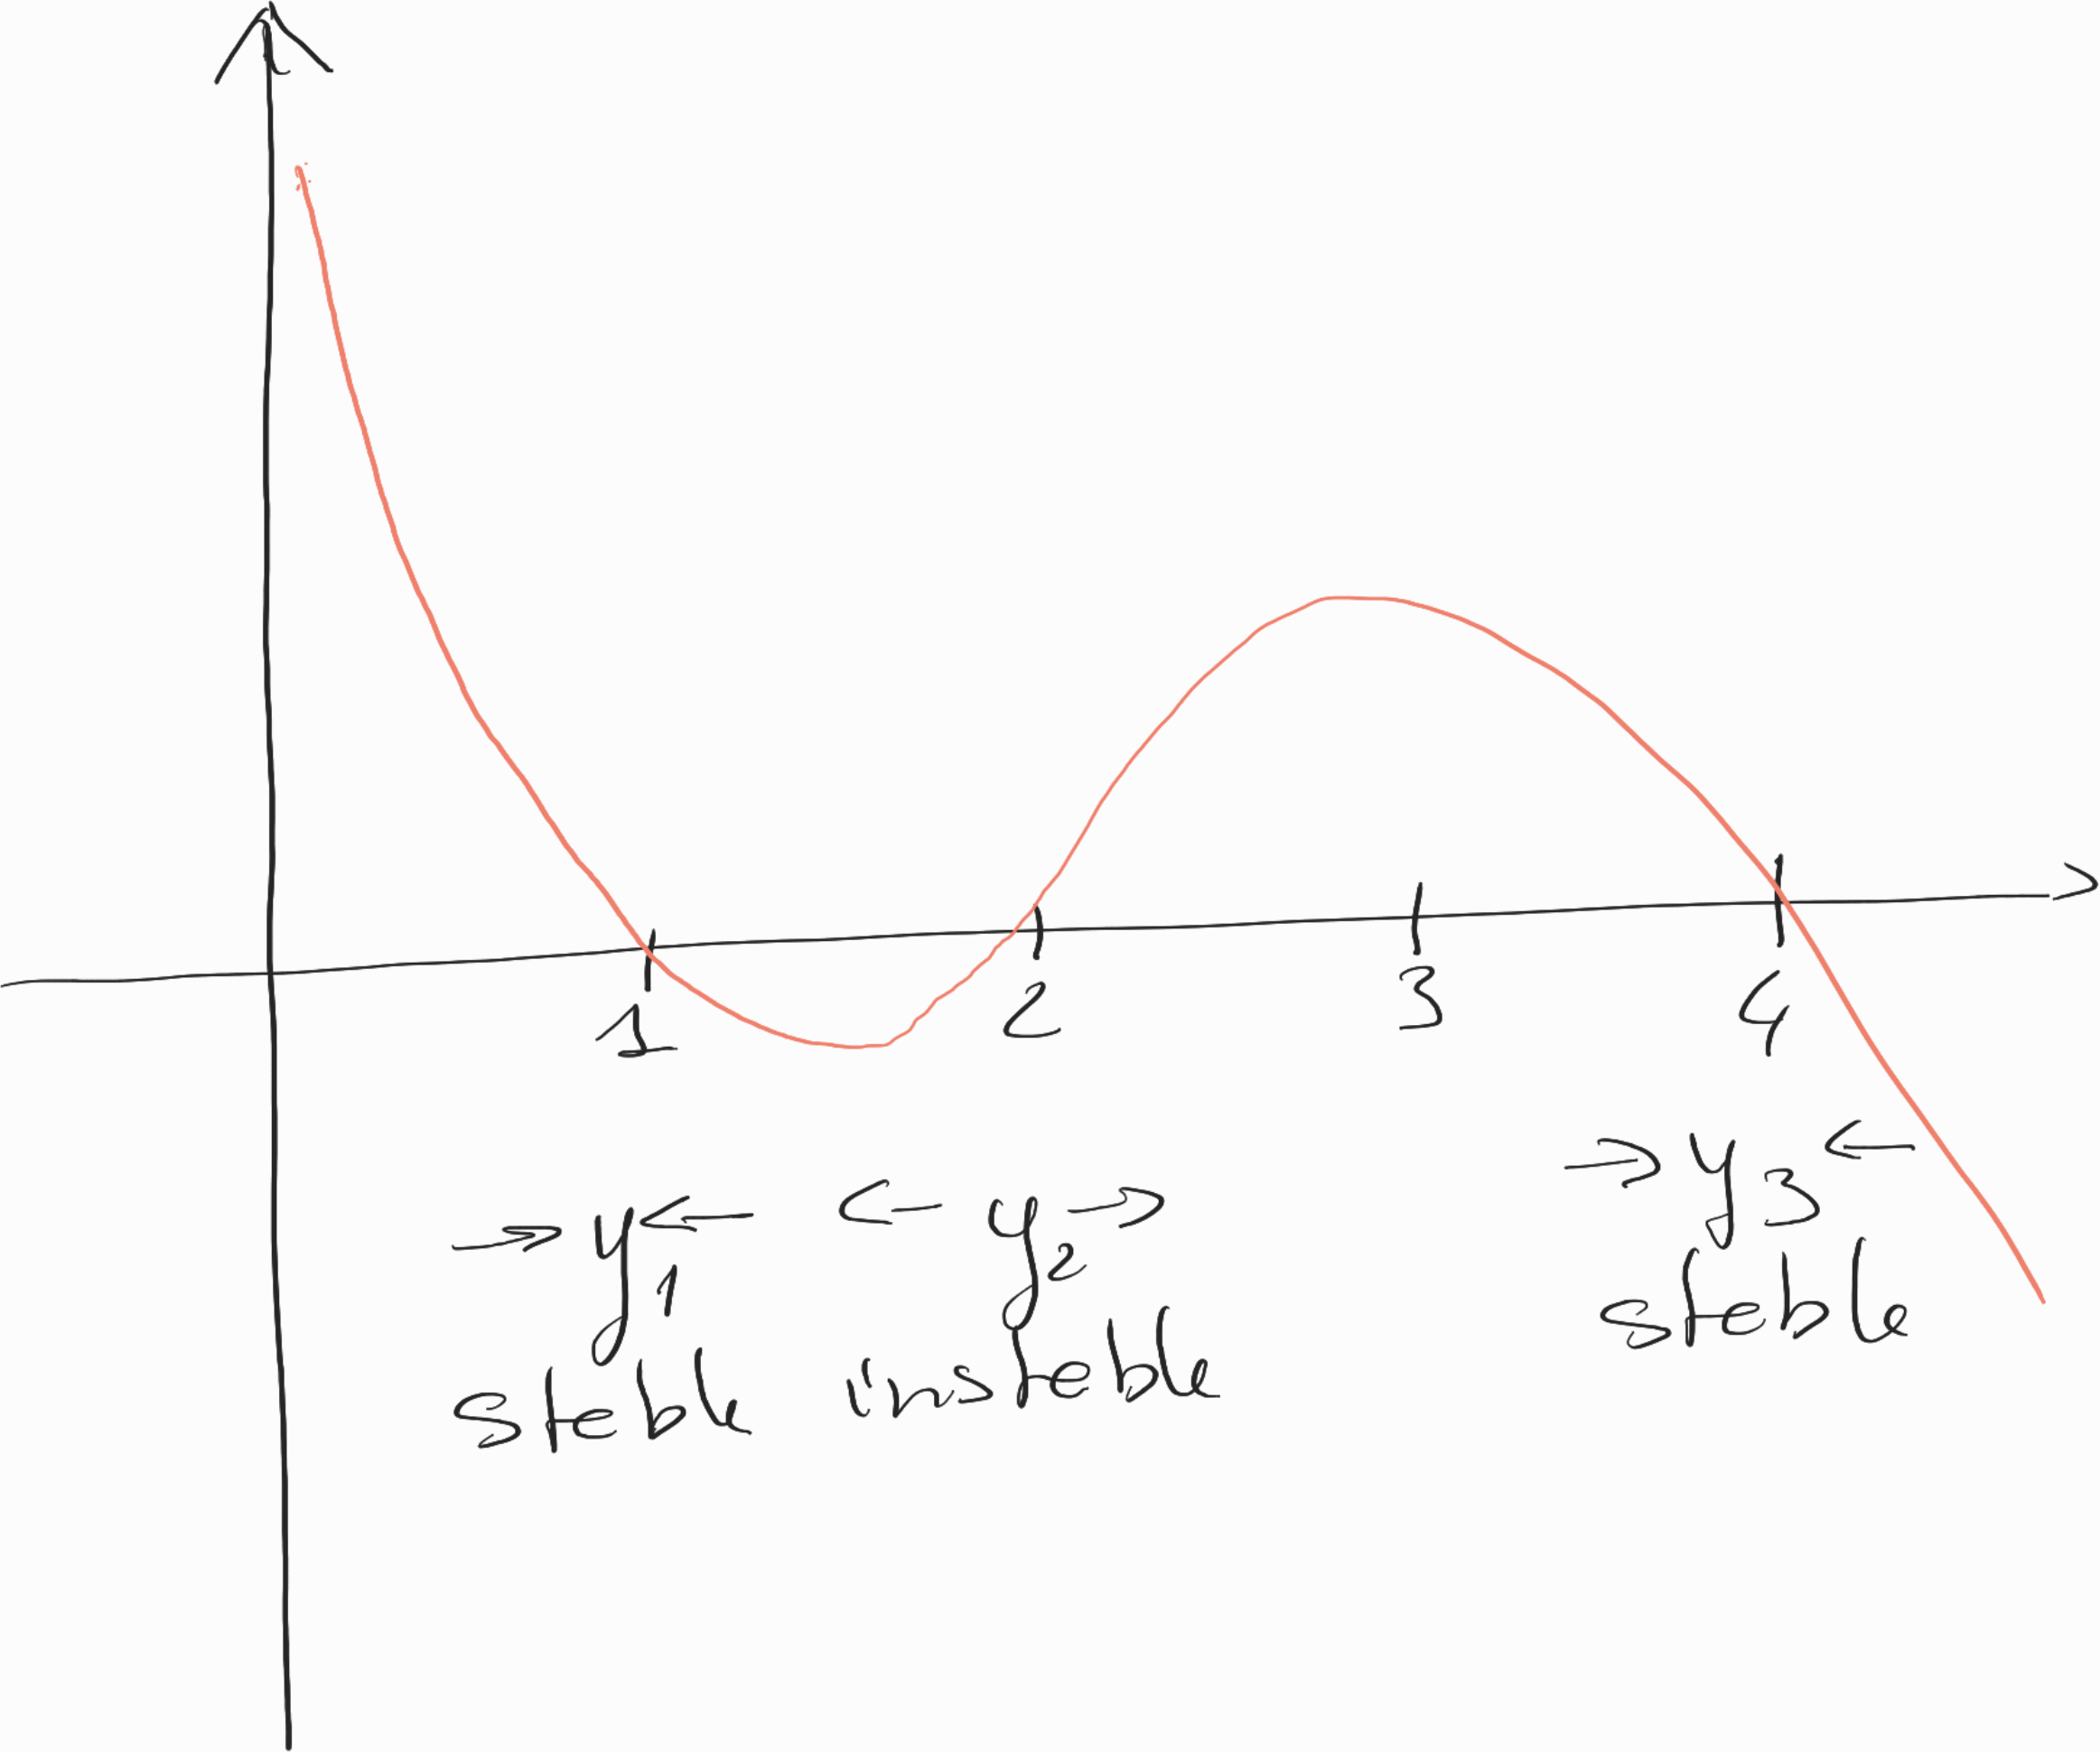
\includegraphics[width=.5\textwidth]{TD-SUbioL3-TD2Exo2}
  $$
}


